
%%%%%%%%%%%%%%%%%%%%%%%%%%%%%%%%%%%%%%%%%
% University/School Laboratory Report
% LaTeX Template
% Version 3.1 (25/3/14)
%
% This template has been downloaded from:
% http:\\www.LaTeXTemplates.com
%
% Original author:
% Linux and Unix Users Group at Virginia Tech Wiki 
% (https:\\vtluug.org/wiki/Example_LaTeX_chem_lab_report)
%
% License:
% CC BY-NC-SA 3.0 (http:\\creativecommons.org/licenses/by-nc-sa/3.0/)
%
%%%%%%%%%%%%%%%%%%%%%%%%%%%%%%%%%%%%%%%%%

%----------------------------------------------------------------------------------------
%	PACKAGES AND DOCUMENT CONFIGURATIONS
%----------------------------------------------------------------------------------------

\documentclass[12pt]{article}
\usepackage{booktabs}
\usepackage{float}
\usepackage{fontspec}
\usepackage{mathtools}
\usepackage{xcolor}
\usepackage{titlesec}
%\usepackage{arial}
\usepackage{mathptmx}
\usepackage[version=3]{mhchem} % Package for chemical equation typesetting
\usepackage{siunitx} % Provides the \SI{}{} and \si{} command for typesetting SI units
\usepackage{graphicx} % Required for the inclusion of images
\usepackage{hyperref}
\usepackage{amsmath} % Required for some math elements 
\usepackage{inputenc}
\usepackage[T1]{fontenc}
%\usepackage[portuguese]{babel}
\usepackage{hyphenat}
\usepackage{helvet}
\usepackage{titlesec}
\usepackage{titling}
\usepackage{setspace}
\usepackage{booktabs}
\usepackage[acronym,nomain,nonumberlist,toc]{glossaries} % 
\usepackage[british,UKenglish,USenglish,american]{babel}

%\hyphenation{mate-mática recu-perar}

\usepackage{etoolbox}

\AtBeginDocument{%
	\setlength{\abovedisplayskip}{6pt}
	\setlength{\belowdisplayskip}{6pt}
}

\setcounter{tocdepth}{6}
\setcounter{secnumdepth}{6}



\makeatletter
\g@addto@macro\normalsize{%
	\setlength\abovedisplayskip{6pt}
	\setlength\belowdisplayskip{6pt}
	\setlength\abovedisplayshortskip{6pt}
	\setlength\belowdisplayshortskip{6pt}
}
\makeatother

\setlength\parindent{0pt} % Removes all indentation from paragraphs

\renewcommand{\labelenumi}{\alph{enumi}.} % Make numbering in the enumerate environment by letter rather than number (e.g. section 6)

\setsansfont{Arial}
% Set serifed font to Cambria
%\setmainfont{Times New Roman}
\setmainfont[SizeFeatures={Size=12}]{Arial}
\newfontfamily\subsubsectionfont{Times New Roman} %12pt large
\newfontfamily\headingfont[]{Arial}
% Set formats for each heading level
\titleformat*{\section}{\Large\bfseries\sffamily}
\titleformat*{\subsection}{\Large\bfseries\sffamily}
\titleformat*{\subsubsection}{\itshape\subsubsectionfont}

\font\myfon=Arial at 17pt
\font\myfont=Arial at 15pt
\font\myfontt=Arial at 12pt

\usepackage{enumitem}
\usepackage{booktabs}
\usepackage{graphicx}


\newfontfamily\capfont[SizeFeatures={Size=10}]{Times New Roman}
\newfontfamily\mathfont[SizeFeatures={Size=12}]{Times New Roman}


\usepackage{caption}
\DeclareCaptionFont{cap}{\capfont}

\makeatletter %only needed in preamble
\renewcommand\scriptsize{\@setfontsize\scriptsize{10pt}{10pt}}
\makeatother
\captionsetup{font=cap, labelfont=cap}

\usepackage{subcaption}
\usepackage{wrapfig}

\renewcommand{\thesection}{\Roman{section}.} 
\renewcommand{\thesubsection}{\thesection\Roman{subsection}}
\renewcommand{\baselinestretch}{1.5} 

\titlespacing*{\section}
{0pt}{6pt}{3pt}

\titlespacing*{\subsection}
{0pt}{6pt}{3pt}

\titlespacing*{\subsubsection}
{0pt}{6pt}{3pt}

%\setmainfont{mathptmx}

\usepackage{geometry}
\geometry{
	a4paper,
	total={170mm,257mm},
	left=20mm,
	top=20mm,
}


\usepackage{spverbatim}


\usepackage{listings}
\lstset{
	keywordstyle=\color{RoyalBlue},
	basicstyle=\small\ttfamily,
	commentstyle=\color{black}\ttfamily,
	%    rulecolor=\color{black},
	showstringspaces=false,
	breaklines=true,
	frameround=ftff,
	frame=single,
	columns=flexible,
	%    belowcaptionskip=5em,
	aboveskip=1.25em,
	language=Verilog,
}

\renewcommand{\lstlistingname}{Code excerpt} 

 \setlength{\belowcaptionskip}{-10pt}





\begin{document}
	
	
	%----------------------------------------------------------------------------------------------------------------------------------------------------------------------------------------------------
	%																					CAPA
	%----------------------------------------------------------------------------------------------------------------------------------------------------------------------------------------------------
	
	%----------------------------------------------------------------------------------------------------------------------------------------------------------------------------------------------------
	%----------------------------------------------------------------------------------------------------------------------------------------------------------------------------------------------------
	\begin{titlepage}
		\begin{figure}
			
\includegraphics[scale=0.4]{IST} 
		\end{figure}
		
		\vspace*{3cm}
		\begin{center}
			\headingfont\Large{\bfseries INSTITUTO SUPERIOR TÉCNICO}\\[2cm]
			\headingfont\LARGE{\bfseries Design Test and Reliability of Electronic Systems \\[1,5cm]Project 1 - Digital Controller}\\[0,5cm]
			%\headingfont\Large{\bfseries RELATÓRIO FORMAL}
		\end{center}
		\vspace{3cm}
		\headingfont\hfill
		\begin{tabular}{@{}l@{}}
		    Group 2\\ 
			n$^{\circ}$ 77973 - Pedro Pina\\
			n$^{\circ}$ 84779 - Afonso Muralha\\
			\\
			Professor Fernando Gonçalves
			
		\end{tabular}
		\vspace{2,5cm}
		\begin{center}
			\today
		\end{center}
	\end{titlepage}
	%----------------------------------------------------------------------------------------------------------------------------------------------------------------------------------------------------
	%																						CAPA
	%----------------------------------------------------------------------------------------------------------------------------------------------------------------------------------------------------
	\newpage

    \tableofcontents

	\newpage



	\section{Introduction and Objectives}
	The goal of this project is to develop a controller that fulfills certain specifications.\\
	The controller must be described in synthesizable Verilog and it must synthesize without any errors or warnings. \\
	To validate the quality of the testbench, the code coverage must be evaluated using the Cadence simulator (Xcelium).
	
	\section{Specifications}
	The controller must synthesize without any errors or warnings.\\
	As for the testbench, the goal should be a code coverage of 100$\%$ for the Block and FSM categories. 
	\begin{figure}[!htb]
        \centering
        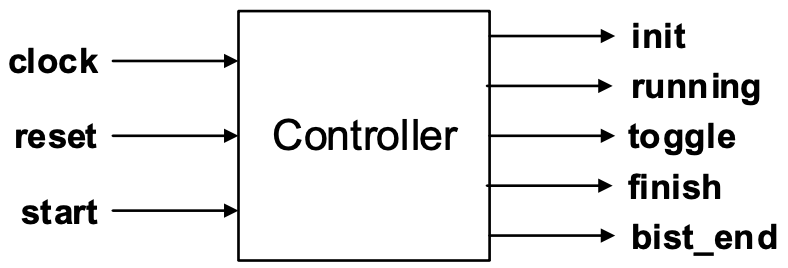
\includegraphics[scale=0.5]{images/controller_interface.png}
            \caption{Controller interface}
            \label{fig:ci}
    \end{figure}
    
	Figure \ref{fig:ci} illustrates the controller interface, with the input and output signals. Every signal has certain sensitivity to the edges and logic levels which must be preserved when building the state machine.\\
    \:
    
	\textbf{Controller inputs}\\
	\emph{clock}: The controller must be sensitive to the rising edges of the clock.\\
	\emph{start}: After a 0→1 transition in this signal, a new sequence must be initiated (see Figure 2). Its value is captured on the rising edge of the clock. While the full sequence is not completed (bist\_end signal set to HIGH), further transitions in the start signal must be ignored.\\
	\emph{reset}: The reset must be synchronous and active at the logic level ‘1’. This signal is used to restart the state machine and the counters, preparing the controller to start a new sequence. When the reset signal goes LOW and the start signal is HIGH, a new sequence must not be restarted. The controller must wait for a 0→1 transition in the start signal to start a new sequence.\\
    \:
    \newpage
	\textbf{Controller outputs}\\
	\emph{init}: This signal is a pulse with a duration of one clock cycle, indicating the start of a new sequence.\\
	\emph{running}: This signal must be HIGH for N clock cycles. If the reset signal goes HIGH, then this signal must go LOW.\\
    \emph{toggle}: This signal must toggle, while the running signal is HIGH.
    \emph{finish}: This signal is a pulse with a duration of one clock cycle, indicating the end of a sequence.\\
    \emph{bist\_end}: This signal must go HIGH when the sequence is completed. The bist\_end signal must go LOW when the reset signal is activated or the start signal has a 0→1 transition.

	
	
	

	
    \section{Digital Controller Design}
	\subsection*{Finite State Machine}
	
	The designed finite state machine features 5 states in order to cop with the specifications mentioned above.
	
	\begin{figure}[!htb]
        \centering
        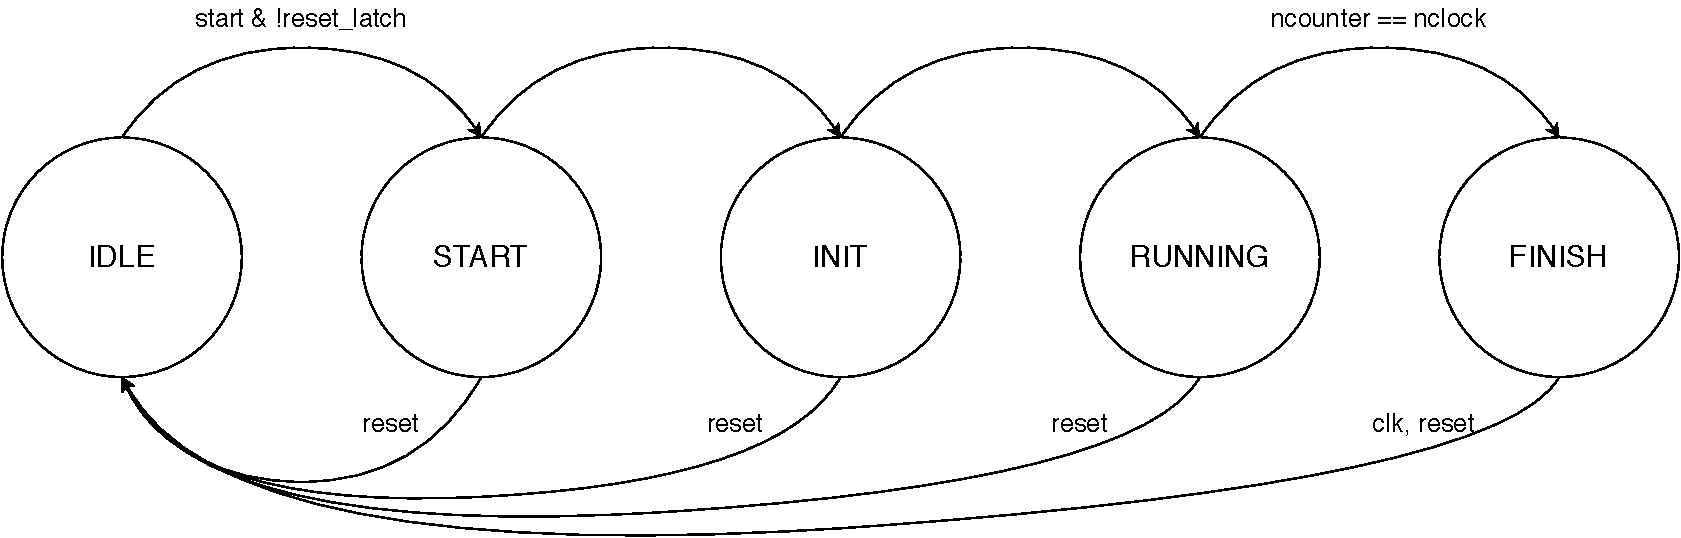
\includegraphics[scale=0.5]{PTFSE_FSM.pdf}
            \caption{Finite state machine diagram.}
            \label{fig:FSMdiagram}
        \end{figure}

    \begin{table}[H]
    \centering
    \caption{Output conditions. More detailed information on state description.}
    \label{tab:outputcond}
    \begin{tabular}{@{}cl@{}}
    \textbf{Outputs} & \textbf{Condition}                                  \\ \midrule
    init             & state == INIT                                                \\
    running          & (state == RUNNING) \& ncounter \textless nclock + 1 \\
    toggle           & (state == RUNNING) \& toggle\_r                     \\
    finish           & state == FINISH                                          \\
    bist\_end        & (complete) \& !(reset | start);                     \\ \bottomrule
    \end{tabular}
    \end{table}
    
    \subsubsection*{IDLE state:}
    This state is activated while waiting for a new sequence to be started. When the start conditions are met, the controller changes into the START state. \newline
    These start conditions are defined by the following logic expression:
    \begin{verbatim}
        start & (state == IDLE) & !reset_latch
    \end{verbatim}
    
    The main drive for the state change is the start pin becoming enabled but in order to meet requirements, a simple reset latch was implemented, so that if the start pin is already enabled on the falling edge of the reset signal, the controller waits for a full transition of the start signal before changing state. This latch was implemented as follows:
    
    \begin{lstlisting}[caption={Reset latch implementation.},captionpos=b]
always @ (posedge start) begin
	if(start & !(reset))
		reset_latch <= 0;
	else
		reset_latch <= 1;
end
    \end{lstlisting}
    
    
    \subsubsection*{START state:}
    On the start stage, the sequence is starting. The controller changes to the INIT state on the following positive clock transition.
    \subsubsection*{INIT state:}
    Whilst on the INIT state, the controller enables the init output and is set to change into \mbox{RUNNING} state on the next positive clock transition.
    \subsubsection*{RUNNING state:}
    On the RUNNING state, the controller generates the toggle and running outputs for the required number of clocks impulses. The number of clock impulses is set by a parameter and, in order to have a suitable sized register to hold the counter variable, the following primitive was used:
    \newpage
    
        \begin{lstlisting}[caption={Creation of the register for the NCLOCK parameter.},captionpos=b]
parameter NCLOCK = 650; //number of clocks for group 2
reg [$clog2(NCLOCK):0] ncounter; //uses the log2 primitive to calculate a suitable size for the register, this is done during compilation.
    \end{lstlisting}
    
    In this state, the running output is enabled, due to the condition:
    \begin{lstlisting}[caption={running output condition.},captionpos=b]
    assign running  = (state == RUNNING) & (ncounter < nclock+1);
    \end{lstlisting}    
    The toggle output is driven by the state and an auxiliary register that carries the output of a toggle process. This process is also responsible for counting the number of elapsed clocks and iterating them.
    \begin{lstlisting}[caption={toggle output condition.},captionpos=b]
    assign toggle   = (state == RUNNING) & toggle_r;
    \end{lstlisting}    
    \begin{lstlisting}[caption={Toggle generator and counter process.},captionpos=b]
always @ (posedge clock) begin
	if(reset | (state == FINISH)) begin
		toggle_r <= 0;
		ncounter <= 0;
	end	
	else if(state == RUNNING) begin
		if(ncounter < NCLOCK) begin
			toggle_r = !toggle_r;
		end
		else begin
			toggle_r <= 0;
		end
		ncounter <= ncounter + 1;
  	end
end
    \end{lstlisting}    
    
    When the iterating register reaches the determined parameter, the state changes to FINISH.
    
    \subsubsection*{FINISH state:}
    Whilst on the FINISH state, the controller enables the finish output and is set to change into IDLE state on the next positive clock transition.
    
    The bist\textunderscore end signal is triggered by the following condition:
    \begin{lstlisting}[caption={bist\textunderscore end register drive.},captionpos=b]
assign bist_end = (complete) & !(reset | start);
    \end{lstlisting}
    

    The complete register is used on order to assure a simultaneous transition of the bist\_end signal. 
    \begin{lstlisting}[caption={Complete register drive.},captionpos=b]
always @ (negedge finish, posedge start, posedge reset) begin
	if(reset | start)
		complete = 0;
	else
		complete = 1;
	
end
\end{lstlisting}
	
	\subsection{Testbench and simulation}
	
	In order to test the controller, a test bench was created. This test bench instances the controller modules and features multiple test scenarios that can be set by commenting the non-relevant tests:
    \begin{lstlisting}[caption={Testbench test set.},captionpos=b]
//===========SET TEST==========
`define normal
`define consequent_test
`define mid_start
`define start_reset
`define mid_reset
    \end{lstlisting}
    
    
    For the following tests, an NCLOCK of 10 was used for easier visualization.
	
	\subsubsection*{Normal test}
	Runs one sequence.
	\begin{figure}[H]
        \centering
        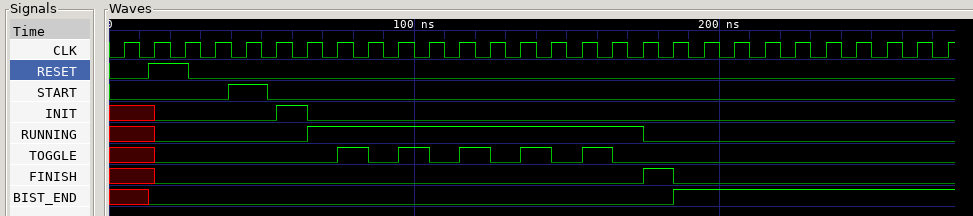
\includegraphics[scale=0.6]{normal_test.png}
            \caption{Normal test waveforms.}
            \label{fig:normal_test}
    \end{figure}
	
	\subsubsection*{Consequent test}
	Runs two sequences in a row:
	\begin{figure}[H]
        \centering
        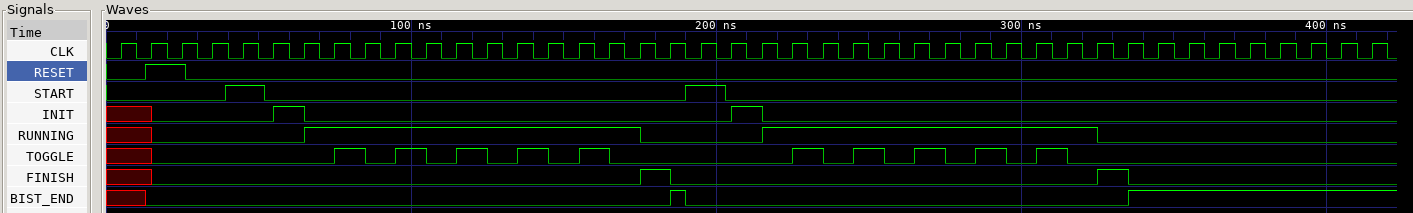
\includegraphics[scale=0.45]{consequent_test.png}
            \caption{Consequent test waveforms.}
            \label{fig:normal_test}
    \end{figure}
	
	\subsubsection*{Mid-sequence start test}
	Runs one sequence and toggles the start during the running sequence. The mid-sequence start should not affect the sequence.
	\begin{figure}[H]
        \centering
        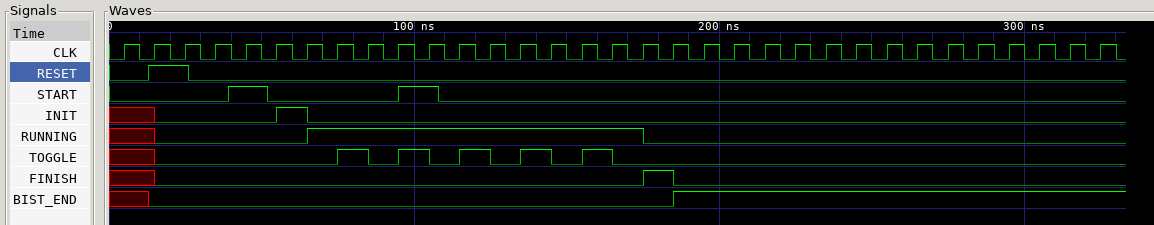
\includegraphics[scale=0.5]{midstart_test.png}
            \caption{Mid-sequence start test waveforms.}
            \label{fig:normal_test}
    \end{figure}
	
	\subsubsection*{Mid-sequence reset test}
	Runs one sequence and toggles the reset during the running sequence and starts a new one after that. The mid-sequence reset should abort the sequence and the following sequence should complete without any issues.
	\begin{figure}[H]
        \centering
        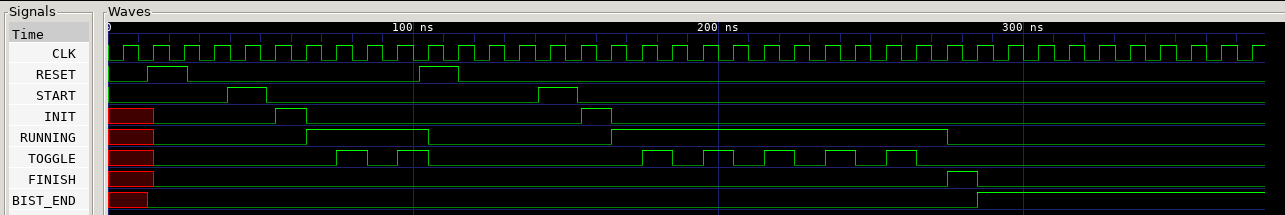
\includegraphics[scale=0.45]{midreset_test.png}
            \caption{Mid-sequence reset test waveforms.}
            \label{fig:normal_test}
    \end{figure}
	
	\subsubsection*{Start/reset latch test}
	Runs one sequence and after its completion, enables the start and reset signals and disables the reset signal. In this case the sequence should not start. After that a toggle of the start signal should start a new sequence and it should complete without issues.
	
	\begin{figure}[H]
        \centering
        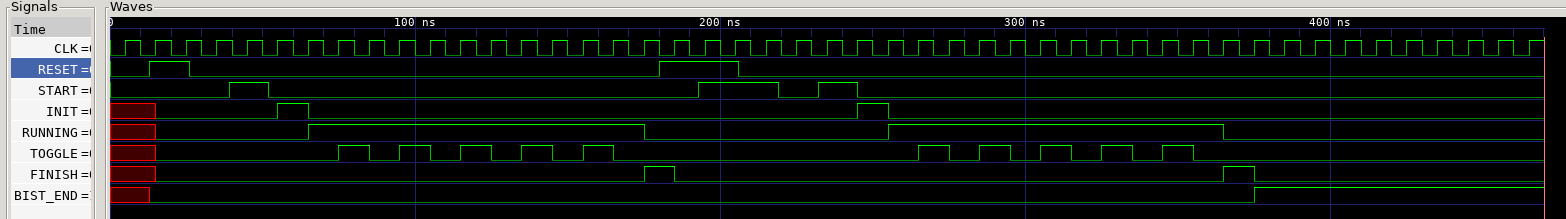
\includegraphics[scale=0.4]{startreset_test.png}
            \caption{Start/reset latch test waveforms.}
            \label{fig:normal_test}
    \end{figure}
	
	In order to validate the running and toggle signals, two counter variables were created on the test bench that are used for measuring then length of the running signal and the number of pulses of the toggle signal.
	    \begin{lstlisting}[caption={Counter variables.},captionpos=b]
integer pulsecount = 0;
integer runningcount = 0;

always @ (posedge TOGGLE) begin
    pulsecount = pulsecount +1; 
end

always @ (posedge CLK) begin
    if(RUNNING)
        runningcount = runningcount + 1;
end
    \end{lstlisting}
    
    These variables are printed and reseted after a sequence:
    \begin{lstlisting}[caption={Conter variable prints.},captionpos=b]
$display("Number of pulses: %d pulses.",pulsecount);
$display("Time of running: %d clock pulses.",runningcount-1); //-1 because the first rising edge of the clock doesent count
pulsecount = 0;
runningcount = 0;
    \end{lstlisting}
    This was tested for multiple NCLOCK values to validate if the method can be trusted for measuring the number of pulses and the length of the running signal. Then, simulating one normal sequence with the NCLOCK set to the group's number (650) we can validate the result with the output of the program:
    \begin{lstlisting}[caption={Toggle and running validation.},captionpos=b]
Number of pulses:           325 pulses.
Time of running:            650 clock pulses.
    \end{lstlisting}    
	
	
    \subsection*{Code Coverage and synthesis validation}
    In order to validate the quality of the produced code, the controller module was synthesized on the Vivado IDE and the report can be found alongside the submitted files.
    
    A code coverage and FSM reports were also generated using cadence tools for the controller using NCLOCK = 650.
    \begin{figure}[H]
        \centering
        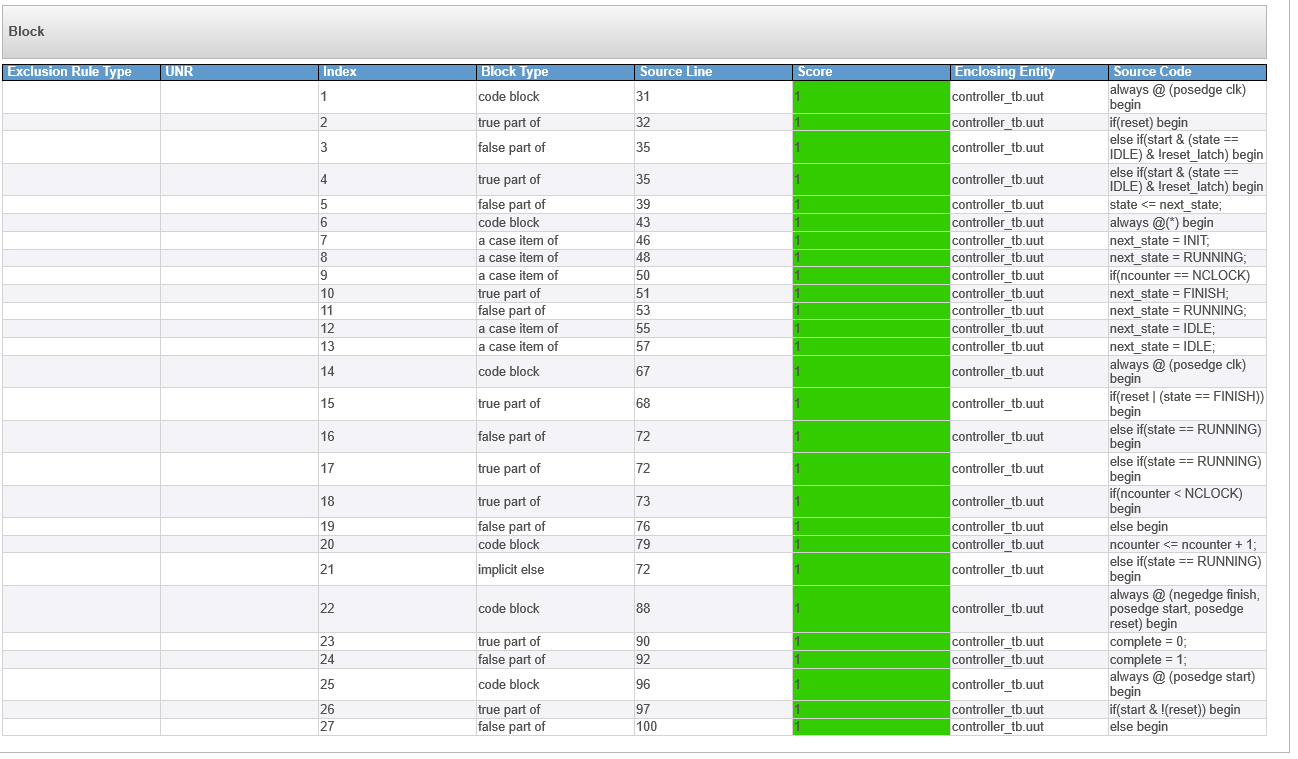
\includegraphics[scale=0.4]{codecoverage.png}
            \caption{Code coverage report.}
            \label{fig:CodeCoverageReport}
    \end{figure}
    \begin{figure}[H]
        \centering
        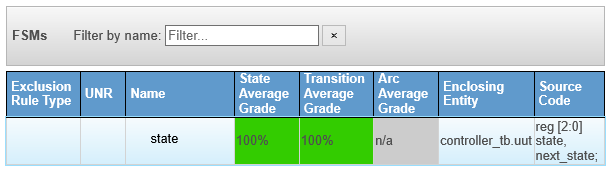
\includegraphics[scale=0.7]{FSM_report1.png}
            \caption{FSM report 1.}
            \label{fig:FSMreport1}
    \end{figure}
    \begin{figure}[H]
        \centering
        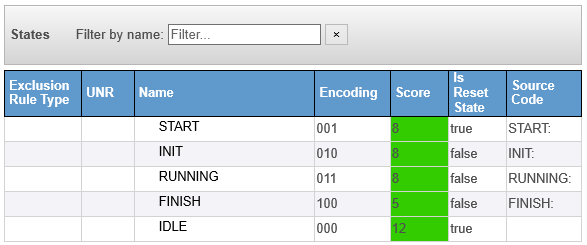
\includegraphics[scale=0.7]{FSM_report2.png}
            \caption{FSM report 2.}
            \label{fig:FSMreport2}
    \end{figure}
    \begin{figure}[H]
        \centering
        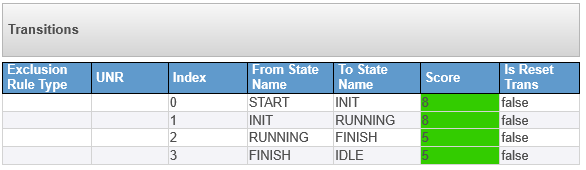
\includegraphics[scale=0.7]{FSM_report3.png}
            \caption{FSM report 3.}
            \label{fig:FSMreport3}
    \end{figure}
    
    
    
 \newpage   
	
	\section{Conclusion}
	This project objective was to learn how to program and develop a controller with certain \mbox{specifications}. This meant that, for it to work properly, the ones developing it, needed to have a clear understanding of every input and ouput signals functionality and behaviour \mbox{- how} does a signal influences other signals and how does it develop throw a specific time period.\\ 
	Therefore, having tools such as the Gtkwave and the Cadence simulator (Xcelium) are important to evaluate the code, which errors and warnings it may have, during the developing stage. In addition to that, having a graphic representation of what has been done can guarantee that the final product is working as intended, with every specification running correctly.

	\begin{thebibliography}{20}
\bibitem{ref1}
Verilog Tutorial (Course slides)\\
\url{https://fenix.tecnico.ulisboa.pt/downloadFile/1126518382240212/My%20Verilog%20Tutorial.pdf}

\end{thebibliography}


\end{document}
